\chapter{Proverb 22}

\begin{figure}
  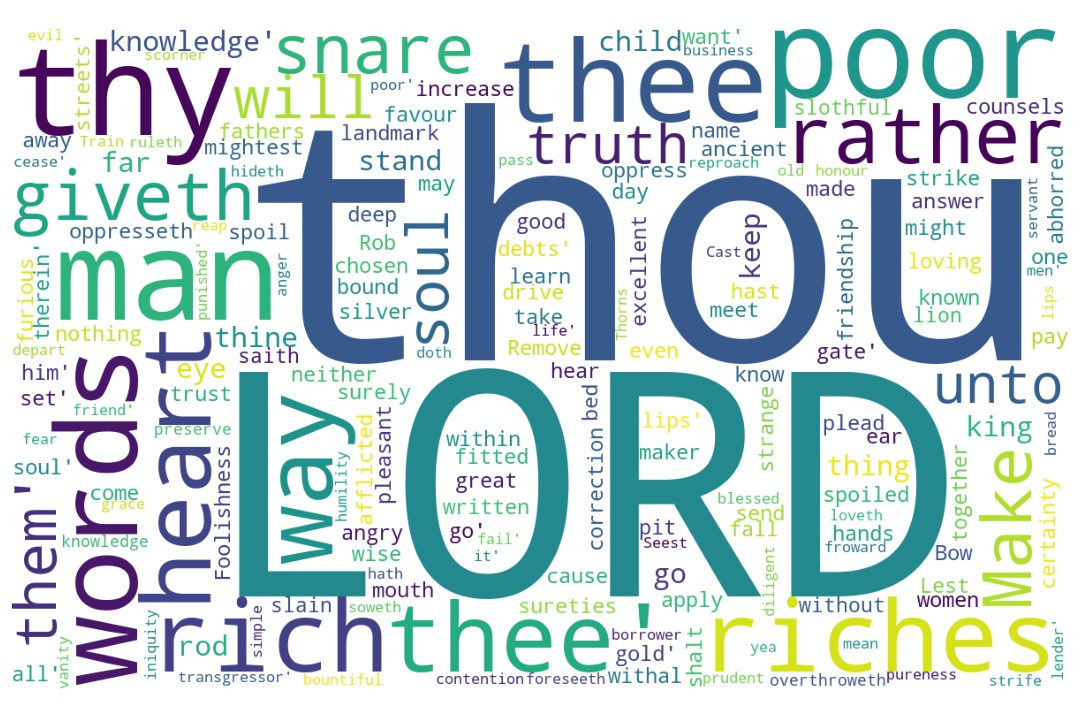
\includegraphics[width=\linewidth]{20OT-Proverbs/Proverb22-WordCloud.jpg}
  \caption{Proverb 22 Word Cloud}
  \label{fig:Proverb 22 word Cloud}
\end{figure}


\marginpar{\scriptsize \centering \fcolorbox{bone}{lime}{\textbf{AN ALL-SEEING GOD}}\\ (Proverb 22:1-29) \begin{compactenum}[I.][8]
    \item \textbf{Are all Around!}(\index[scripture]{Proverbs!Pro 05:21}  \index[scripture]{Proverbs!Pro 15:03}  \index[scripture]{Zechariah!Zch 04:10} (Pro 5:21, Pro 15:3, Zech 4:10)
    \item \textbf{Appraise the Situation} \index[scripture]{1 Kings!1Kng 16:25} \index[scripture]{2 Chronicles!2Chr 14:2}  \index[scripture]{2 Chronicles!2 Chr 21:06}  \index[scripture]{2 Chronicles!2 Chr 29:06} (1Kng 16:25, 2Chr 14:2, 2Chr 21:16, 2Chr 29:6)
    \item \textbf{Are Active} \index[scripture]{Proverbs!Pro 22:12} (Pro 22:12)
    \item \textbf{Approve} \index[scripture]{2 Samuel!2 Sam 15:25} \index[scripture]{Isaiah!Isa 49:05} (2Sam 15:25, Isa 49:5)
    \item \textbf{Are Attentive} (\index[scripture]{Genesis!Gen 6:8}Genesis 06:08, \index[scripture]{2 Chronicles!2 Chr 16:09}2 Chronicles 16:9, \index[scripture]{Psalm!Psa 34:15}Psa 34:15, \index[scripture]{1 Peter!1Pet 03:12}1Pet 3:12)
    \item \textbf{Are Aware} \index[scripture]{Zechariah!Zech 04:10} (Zech 4:10)
    \item \textbf{Analyze} \index[scripture]{Amos!Amo 09:08} (Amos 9:8)
\end{compactenum}}

\marginpar{\scriptsize \centering \fcolorbox{bone}{yellow}{\textbf{SOME ADVICE}}\\ (Proverb 22:1-29) \begin{compactenum}[I.][8]
    \item \textbf{Choice} \index[scripture]{Proverbs!Pro 22:01} (Pro 22:1)
    \item \textbf{Child} \index[scripture]{Proverbs!Pro 22:06}\index[scripture]{Proverbs!Pro 22:15} (Pro 22:6, 15)
    \item \textbf{Contention} \index[scripture]{Proverbs!Pro 22:10} (Pro 22:10)
    \item \textbf{Correction} \index[scripture]{Proverbs!Pro 22:15} (Pro 22:15)
    \item \textbf{Counsels} \index[scripture]{Proverbs!Pro 22:20} (Pro 22:20)
    \item \textbf{Certainty} \index[scripture]{Proverbs!Pro 22:21} (Pro 22:21)
    \item \textbf{Cause} \index[scripture]{Proverbs!Pro 22:23} (Pro 22:23)
\end{compactenum}}

\footnote{\textcolor[cmyk]{0.99998,1,0,0}{\hyperlink{TOC}{Return to end of Table of Contents.}}}\footnote{\href{https://audiobible.com/bible/proverbs_22.html}{\textcolor[cmyk]{0.99998,1,0,0}{Proverbs Audio}}}\textcolor[cmyk]{0.99998,1,0,0}{A \emph{good} name \emph{is} rather to be \fcolorbox{bone}{lime}{chosen} than great riches, \emph{and} loving favour rather than silver and gold.}
[2] \textcolor[cmyk]{0.99998,1,0,0}{The rich and poor meet together: the LORD \emph{is} the maker of them all.}
[3] \textcolor[cmyk]{0.99998,1,0,0}{A prudent \emph{man} foreseeth the evil, and hideth himself: but the simple pass on, and are punished.}
[4] \textcolor[cmyk]{0.99998,1,0,0}{By humility \emph{and} the fear of the LORD \emph{are} riches, and honour, and life.}
[5] \textcolor[cmyk]{0.99998,1,0,0}{Thorns \emph{and} snares \emph{are} in the way of the froward: he that doth keep his soul shall be far from them.}
[6] \textcolor[cmyk]{0.99998,1,0,0}{Train up a \fcolorbox{bone}{lime}{child} in the way he should go: and when he is old, he will not depart from it.}
[7] \textcolor[cmyk]{0.99998,1,0,0}{The rich ruleth over the poor, and the borrower \emph{is} servant to the lender.}
[8] \textcolor[cmyk]{0.99998,1,0,0}{He that soweth iniquity shall reap vanity: and the rod of his anger shall fail.}
[9] \textcolor[cmyk]{0.99998,1,0,0}{He that hath a bountiful eye shall be blessed; for he giveth of his bread to the poor.}\footnote{See Proverbs 21:26 and 14:21. The Roman Vulgate and Alexandrian Septuagint add about eleven to fifteen words not found in the Bible and prove, again, that “Western” and “Alexandrian” manuscripts for the New Testament have the same type of writers, admirers, “preservers,” and believers. For 22:9, the LXX has: ``He that has pity on the poor shall himself be maintained; for he has given of his own bread to the poor. He that gives liberally secures victory an honour; but he takes away the life of them that posses.''}\footnote{\textbf{Proverb 14:21} - He that despiseth his neighbour sinneth: but he that hath mercy on the poor, happy is he.}\footnote{\textbf{Proverb 21:26} - He coveteth greedily all the day long: but the righteous giveth and spareth not.}
[10] \textcolor[cmyk]{0.99998,1,0,0}{Cast out the scorner, and \fcolorbox{bone}{lime}{contention} shall go out; yea, strife and reproach shall cease.}
[11] \textcolor[cmyk]{0.99998,1,0,0}{He that loveth pureness of heart, \emph{for} the grace of his lips the king \emph{shall} \emph{be} his friend.}\footnote{The proverb is clear; especially so in the light of Matthew 5:8 and 2 Samuel 22:27 (see further comment under 21:8). Since God is pure (Hab. 1:13) and the word of God is pure (Psa. 119:140), the “king” (see comments under 20:2, 8 and 21:1) will accept the “pure in heart.” “For the grace of his lips” implies that the pure in heart speaks out of the abundance of his heart (Matt. 5:8). These “lips” are found again in Proverbs 8:6, 10:13, 10:21, 32, 12:19, 14:3, 15:7, and 16:10.}
[12] \textcolor[cmyk]{0.99998,1,0,0}{The eyes of the LORD preserve knowledge, and he overthroweth the words of the transgressor.}
[13] \textcolor[cmyk]{0.99998,1,0,0}{The slothful \emph{man} saith, \emph{There} \emph{is} a lion without, I shall be slain in the streets.}
[14] \textcolor[cmyk]{0.99998,1,0,0}{The mouth of strange women \emph{is} a deep pit: he that is abhorred of the LORD shall fall therein.}
[15] \textcolor[cmyk]{0.99998,1,0,0}{Foolishness \emph{is} bound in the heart of a \fcolorbox{bone}{lime}{child}; \emph{but} the rod of \fcolorbox{bone}{lime}{correction} shall drive it far from him.}
[16] \textcolor[cmyk]{0.99998,1,0,0}{He that oppresseth the poor to increase his \emph{riches,} \emph{and} he that giveth to the rich, \emph{shall} surely \emph{come} to want.}
[17] \textcolor[cmyk]{0.99998,1,0,0}{Bow down thine ear, and hear the words of the wise, and apply thine heart unto my knowledge.}
[18] \textcolor[cmyk]{0.99998,1,0,0}{For \emph{it} \emph{is} a pleasant thing if thou keep them within thee; they shall withal be fitted in thy lips.}
[19] \textcolor[cmyk]{0.99998,1,0,0}{That thy trust may be in the LORD, I have made known to thee this day, even to thee.}
[20] \textcolor[cmyk]{0.99998,1,0,0}{Have not I written to thee excellent things in \fcolorbox{bone}{lime}{counsels} and knowledge,}
[21] \textcolor[cmyk]{0.99998,1,0,0}{That I might make thee know the \fcolorbox{bone}{lime}{certainty} of the words of truth; that thou mightest answer the words of truth to them that send unto thee?}
[22] \textcolor[cmyk]{0.99998,1,0,0}{Rob not the poor, because he \emph{is} poor: neither oppress the afflicted in the gate:}
[23] \textcolor[cmyk]{0.99998,1,0,0}{For the LORD will plead their \fcolorbox{bone}{lime}{cause}, and spoil the soul of those that spoiled them.}
[24] \textcolor[cmyk]{0.99998,1,0,0}{Make no friendship with an angry man; and with a furious man thou shalt not go:}
[25] \textcolor[cmyk]{0.99998,1,0,0}{Lest thou learn his ways, and get a snare to thy soul.}
[26] \textcolor[cmyk]{0.99998,1,0,0}{Be not thou \emph{one} of them that strike hands, \emph{or} of them that are sureties for debts.}
[27] \textcolor[cmyk]{0.99998,1,0,0}{If thou hast nothing to pay, why should he take away thy bed from under thee?}
[28] \textcolor[cmyk]{0.99998,1,0,0}{Remove not the ancient landmark, which thy fathers have set.}\footnote{\textbf{Deuteronomy 19:14} - Thou shalt not remove thy neighbour’s landmark, which they of old time have set in thine inheritance, which thou shalt inherit in the land that the LORD thy God giveth thee to possess it.}\footnote{\textbf{Deuteronomy 27:17} - Cursed be he that removeth his neighbour’s landmark. And all the people shall say, Amen.}\footnote{\textbf{Proverb 23:10} - Remove not the old landmark; and enter not into the fields of the fatherless:}
[29] \textcolor[cmyk]{0.99998,1,0,0}{Seest thou a man diligent in his business? he shall stand before kings; he shall not stand before mean \emph{men}.}\footnote{\textbf{Proverb 21:5} - he thoughts of the diligent tend only to plenteousness; but of every one that is hasty only to want.}\footnote{\textbf{Proverb 27:23} - Be thou diligent to know the state of thy flocks, and look well to thy herds.}\footnote{\textbf{2 Peter 3:14} - Wherefore, beloved, seeing that ye look for such things, be diligent that ye may be found of him in peace, without spot, and blameless.}


